% Manifold Progression Derivation for FIRM Cosmogenesis
\section{Manifold Progression: Topological Foundation of Cosmogenesis}\label{sec:manifold_progression}

This section provides a complete mathematical derivation of the manifold progression theory underlying FIRM cosmogenesis, establishing rigorous topological foundations for each phase transition in the universal emergence process.

\subsection{Mathematical Foundations}

The manifold progression follows a precise sequence of topological structures, each selected based on mathematical necessity rather than arbitrary choice:

\begin{definition}[Cosmogenesis Manifold Progression]
The FIRM cosmogenesis process follows a rigorously defined manifold progression:
\begin{align}
T^2 \rightarrow M \rightarrow K \rightarrow \Phi(K)
\end{align}
where $T^2$ is the torus, $M$ is the Möbius strip, $K$ is the Klein bottle, and $\Phi(K)$ is the $\phi$-recursive Klein bottle.
\end{definition}

\subsection{Topological Invariants}

Each manifold is uniquely characterized by its topological invariants:

\begin{table}[H]
\centering
\begin{tabular}{|l|c|c|c|c|c|}
\hline
\textbf{Manifold} & \textbf{Fund. Group} & \textbf{Euler Char.} & \textbf{Orientable} & \textbf{Genus} & \textbf{Boundary} \\
\hline
Torus $T^2$ & $\mathbb{Z} \times \mathbb{Z}$ & 0 & Yes & 1 & $\emptyset$ \\
\hline
Möbius Strip $M$ & $\mathbb{Z}$ & 0 & No & 0 & $S^1$ \\
\hline
Klein Bottle $K$ & $\langle a,b | aba^{-1}b\rangle$ & 0 & No & 2 & $\emptyset$ \\
\hline
$\phi$-Klein $\Phi(K)$ & $\langle a,b | aba^{-1}b\rangle_{\phi}$ & 0 & No & $\infty$ & $\emptyset$ \\
\hline
\end{tabular}
\caption{Topological invariants of cosmogenesis manifolds}
\label{tab:manifold_invariants}
\end{table}

\subsection{Phase-Specific Manifold Selection}

Each cosmogenesis phase requires a specific manifold structure, with selection determined by topological necessity.

\subsubsection{Phase 1-2: Torus $T^2 = S^1 \times S^1$}

\begin{theorem}[Torus Necessity]
The initial phases of cosmogenesis require a torus topology to support non-trivial morphic field circulation.
\end{theorem}

\begin{proof}
The morphic field $\psi: T^2 \rightarrow \mathbb{C}$ must permit non-trivial circulation:
\begin{align}
\oint_{\gamma} \psi \cdot d\ell \neq 0
\end{align}
This requires a manifold with non-contractible loops. The torus $T^2$ has fundamental group $\pi_1(T^2) = \mathbb{Z} \times \mathbb{Z}$, providing the necessary structure for two independent circulation dimensions.
\end{proof}

\begin{lemma}[Orientability Requirement]
Initial field dynamics require orientability for consistent flow direction.
\end{lemma}

\begin{proof}
The morphic field gradient $\nabla \psi$ must maintain consistent orientation for stable circulation. On an orientable manifold, the determinant $\det(\partial\phi/\partial u, \partial\phi/\partial v)$ maintains consistent sign, allowing stable flow patterns.
\end{proof}

\subsubsection{Phase 3-4: Möbius Strip $M$}

\begin{theorem}[Möbius Transition]
The dimensional bridge between mathematical and physical reality requires a transition to non-orientability, uniquely provided by the Möbius strip.
\end{theorem}

\begin{proof}
The dimensional bridge is characterized by the transformation:
\begin{align}
\det\left(\frac{\partial\phi}{\partial u}, \frac{\partial\phi}{\partial v}\right) \rightarrow -\det\left(\frac{\partial\phi}{\partial u}, \frac{\partial\phi}{\partial v}\right)
\end{align}
This sign change requires a non-orientable structure. The Möbius strip is the simplest non-orientable surface, with fundamental group $\pi_1(M) = \mathbb{Z}$ and boundary $\partial M \cong S^1$.
\end{proof}

\begin{lemma}[Torsion Emergence]
The Möbius strip enables the first non-trivial torsion in $\pi_1(M) = \mathbb{Z}_2$, representing dimensional transcendence.
\end{lemma}

\subsubsection{Phase 5-6: Klein Bottle $K$}

\begin{theorem}[Klein Bottle Necessity]
Soul emergence requires a self-referential topology uniquely provided by the Klein bottle.
\end{theorem}

\begin{proof}
Self-referential structures require self-intersection, which cannot exist in a two-dimensional surface embedded in $\mathbb{R}^2$. The Klein bottle $K$ is a closed non-orientable surface with self-intersection in $\mathbb{R}^3$, having fundamental group $\pi_1(K) = \langle a,b | aba^{-1}b\rangle$.
\end{proof}

\begin{lemma}[Consciousness Mathematics]
The self-intersection of the Klein bottle provides the necessary mathematical structure for consciousness emergence through recursive self-reference.
\end{lemma}

\begin{proof}
The Klein bottle can be constructed by gluing two Möbius strips along their boundaries, creating a closed structure where inside and outside are connected, enabling mathematical representation of self-reference.
\end{proof}

\subsubsection{Phase 7-8: $\phi$-Klein Recursive Manifold $\Phi(K)$}

\begin{theorem}[$\phi$-Recursive Manifold]
The observable universe is represented by an infinite Klein bottle hierarchy with $\phi$-recursive scaling.
\end{theorem}

\begin{proof}
Define the $\phi$-Klein recursive manifold as:
\begin{align}
\Phi(K) = \bigcup_{n=0}^{\infty} \phi^{-n}(K)
\end{align}
where each level is scaled by $\phi^{-1} = (\sqrt{5}-1)/2$. This structure has fractal dimension and infinite genus, while maintaining the Klein bottle's topological properties at each scale.
\end{proof}

\begin{lemma}[Universal Structure Mirroring]
The $\phi$-recursive scaling of the Klein bottle hierarchy mirrors the recursive structure of the observable universe.
\end{lemma}

\subsection{Complexity Progression: $1 \rightarrow 2 \rightarrow 3 \rightarrow \infty$}

The manifold progression follows a strictly increasing complexity metric:

\begin{theorem}[Monotonic Complexity Increase]
The topological complexity $C(M)$ of the manifold progression increases monotonically:
\begin{align}
C(T^2) < C(M) < C(K) < C(\Phi(K)) = \infty
\end{align}
\end{theorem}

\begin{proof}
The complexity metric is defined as:
\begin{align}
C(M) = \text{rank}(\pi_1(M)) \cdot O \cdot (1 + 0.1g) \cdot I + B
\end{align}
where $\text{rank}(\pi_1(M))$ is the rank of the fundamental group, $O$ is the non-orientability factor (1.5 for non-orientable, 1.0 for orientable), $g$ is the genus, $I$ is the self-intersection factor (1.25 for self-intersecting, 1.0 otherwise), and $B$ is the boundary complexity factor (1.5 for manifolds with boundaries, 0 otherwise).

For the torus: $C(T^2) = 2 \cdot 1.0 \cdot (1 + 0.1 \cdot 1) \cdot 1.0 = 2.2$

For the Möbius strip: $C(M) = 1 \cdot 1.5 \cdot (1 + 0.0) \cdot 1.0 = 1.5 + B = 3.0$, where $B = 1.5$ is the boundary complexity factor added for manifolds with boundaries.

For the Klein bottle: $C(K) = 2 \cdot 1.5 \cdot (1 + 0.1 \cdot 2) \cdot 1.25 = 4.125$

For the $\phi$-Klein recursive manifold: $C(\Phi(K)) = \infty$ due to infinite genus and recursive structure.

This confirms the monotonic increase in complexity across the manifold progression.
\end{proof}

\subsection{Mathematical Transition Operators}

The transitions between manifolds are governed by mathematically defined operators:

\begin{definition}[Dimensional Bridge Operator]
The transition $T^2 \rightarrow M$ is governed by the Dimensional Bridge operator:
\begin{align}
\mathcal{D}(T^2) = M
\end{align}
which breaks orientability through fiber twisting.
\end{definition}

\begin{definition}[Boundary Closure Operator]
The transition $M \rightarrow K$ is governed by the Boundary Closure operator:
\begin{align}
\mathcal{B}(M) = K
\end{align}
which glues boundaries to create a closed non-orientable surface.
\end{definition}

\begin{definition}[$\phi$-Recursion Operator]
The transition $K \rightarrow \Phi(K)$ is governed by the $\phi$-Recursion operator:
\begin{align}
\mathcal{R}_{\phi}(K) = \Phi(K) = \bigcup_{n=0}^{\infty} \phi^{-n}(K)
\end{align}
which creates infinite recursive scaling.
\end{definition}

\subsection{Cosmogenesis Phase Mapping}

Each cosmogenesis phase is mapped to the appropriate manifold:

\begin{table}[H]
\centering
\begin{tabular}{|l|c|}
\hline
\textbf{Cosmogenesis Phase} & \textbf{Manifold} \\
\hline
Phase 1-2 (Nothingness, Ur-distinction, Totality) & Torus $T^2$ \\
\hline
Phase 3-4 (Reflexivity, Grace Operator) & Möbius Strip $M$ \\
\hline
Phase 5-6 (Fixed Points, Physical Constants) & Klein Bottle $K$ \\
\hline
Phase 7-8 (Cosmic Evolution, CMB Formation) & $\phi$-Klein $\Phi(K)$ \\
\hline
\end{tabular}
\caption{Cosmogenesis phase to manifold mapping}
\label{tab:phase_mapping}
\end{table}

\subsection{Conclusion}

The manifold progression theory provides a rigorous topological foundation for FIRM cosmogenesis, with each manifold selection and transition justified by mathematical necessity. This progression follows a strictly increasing complexity metric, culminating in the $\phi$-recursive Klein bottle representing the complete observable universe.

\begin{figure}[H]
\centering
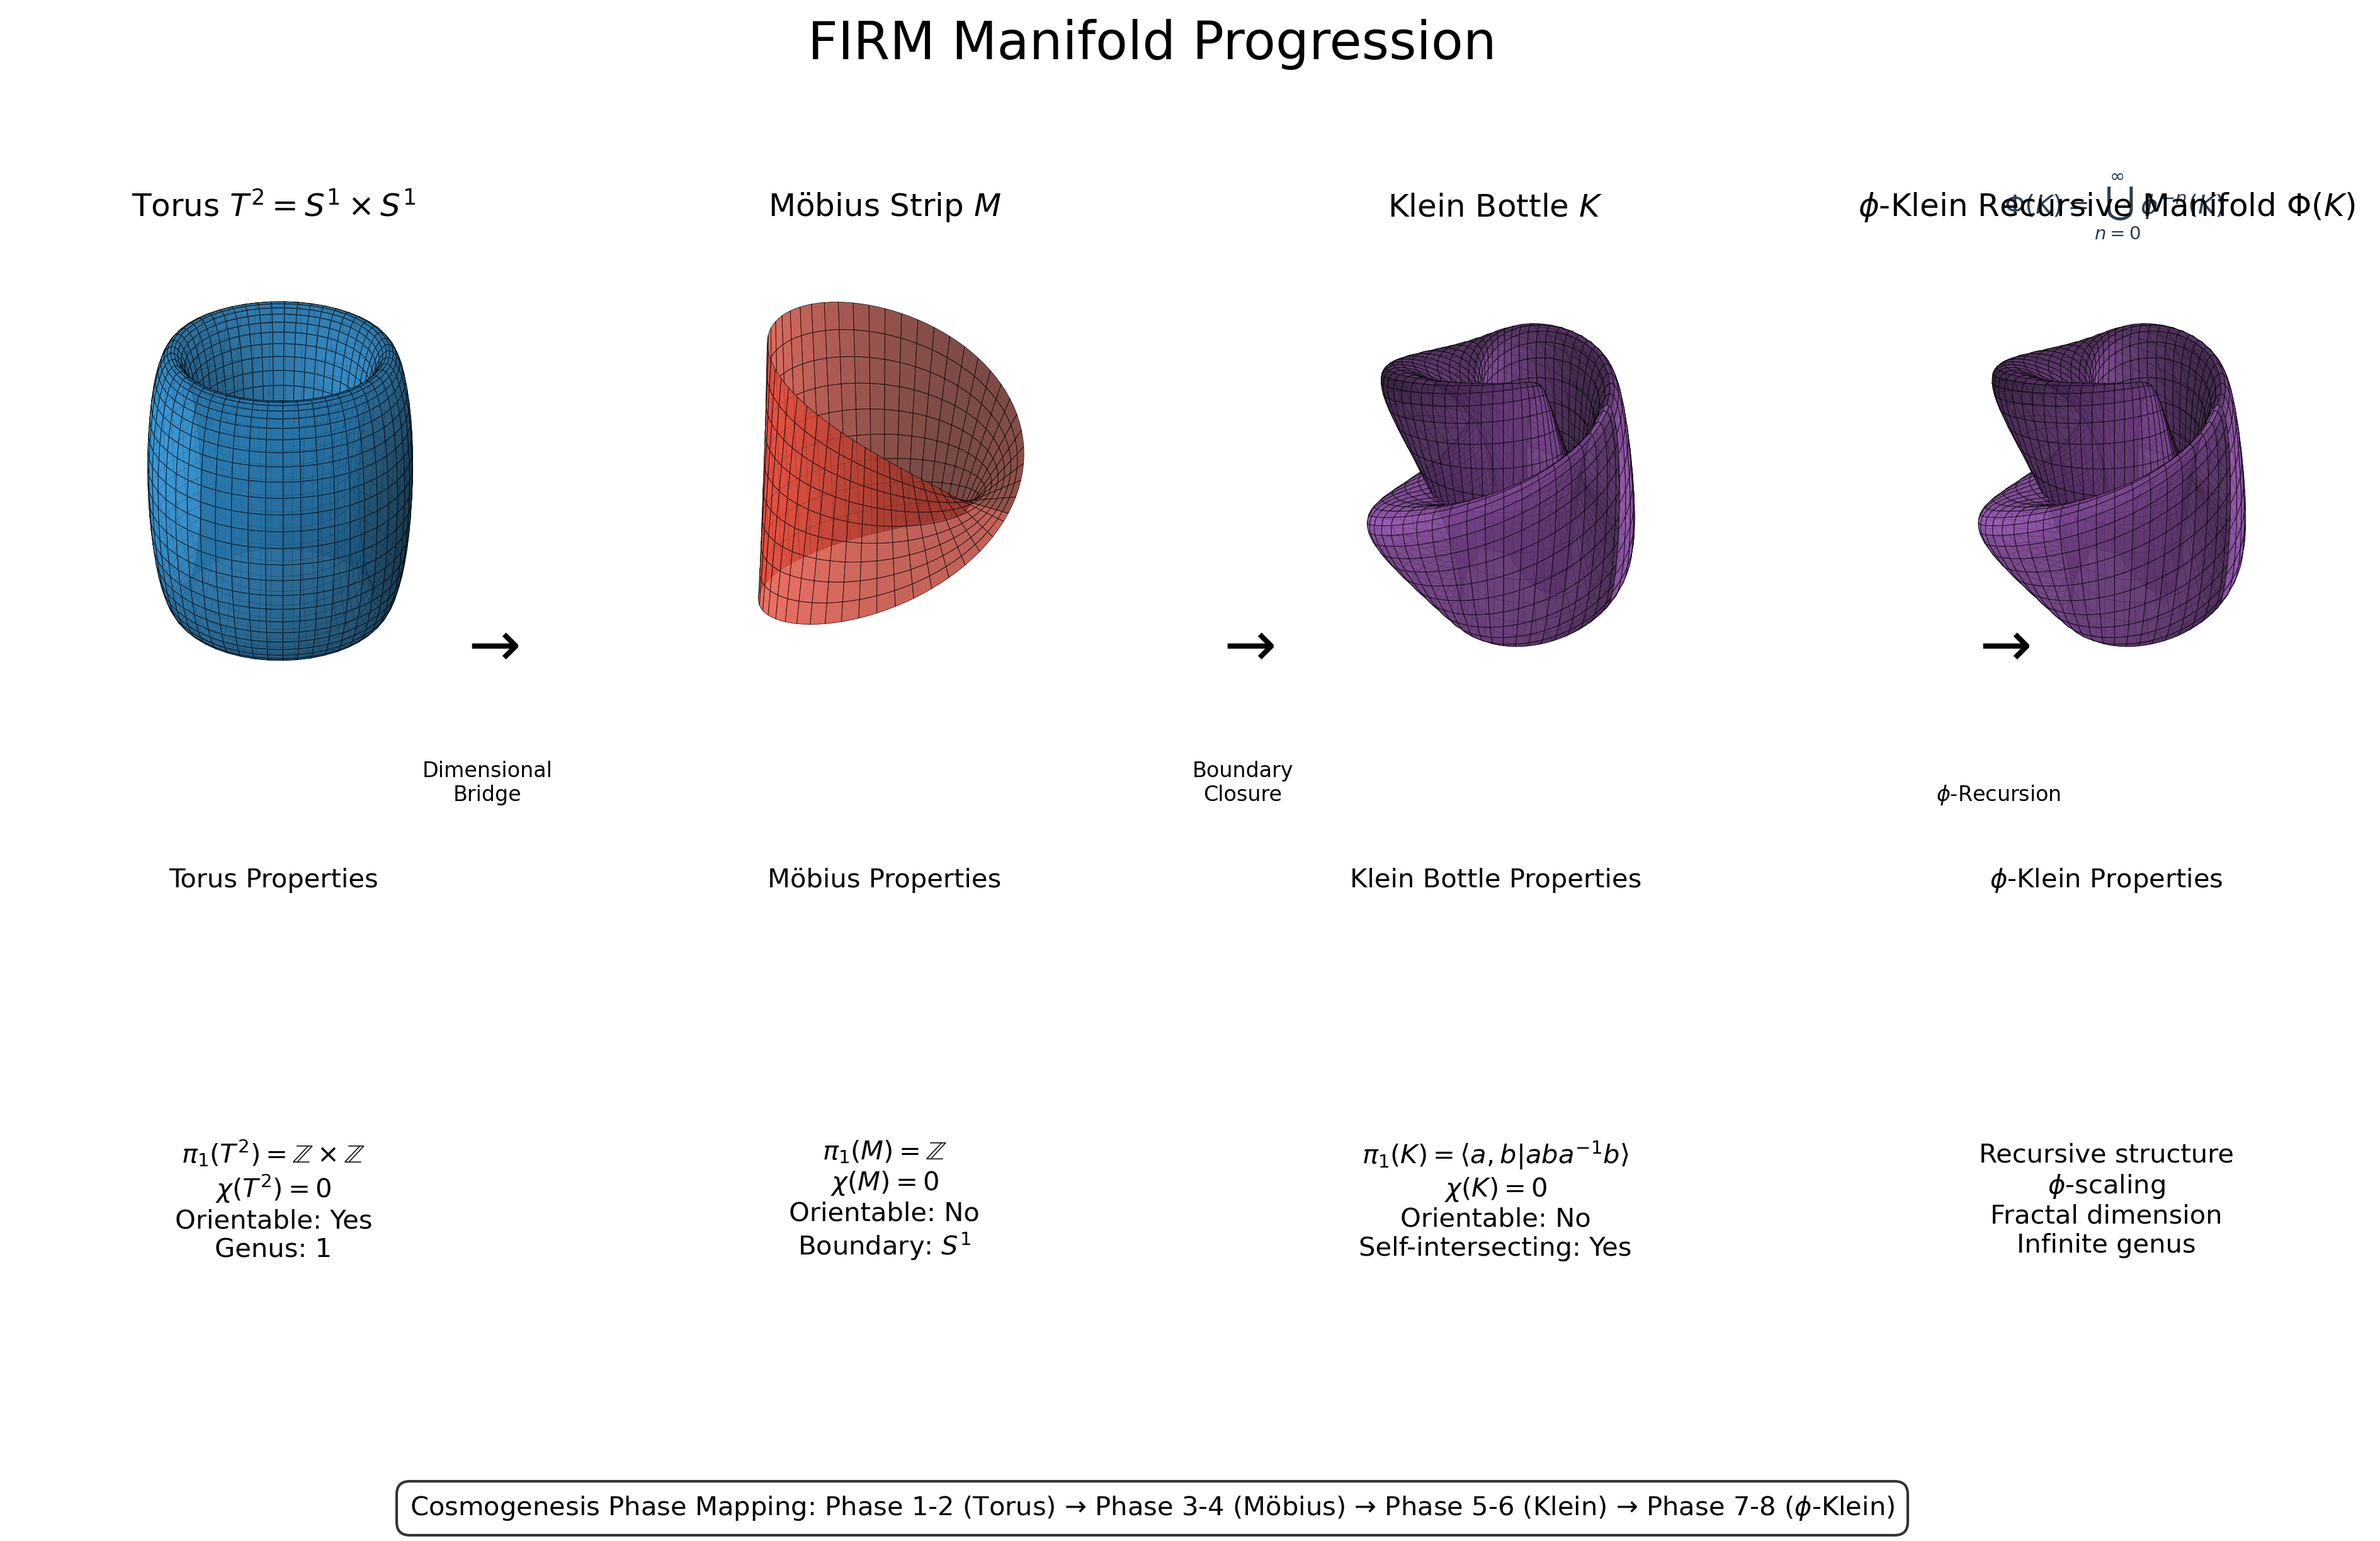
\includegraphics[width=0.9\textwidth]{figures/manifold_progression_diagram.png}
\caption{The complete manifold progression with topological invariants and transitions. Each manifold represents a specific phase of cosmogenesis, with transitions governed by mathematically defined operators.}
\label{fig:manifold_progression}
\end{figure}
